\heading{电动力学-25秋-期末}

\begin{question}[海水到空气的全反射与倏逝波]
海水的相对介电常数为 $\varepsilon_r=4$，一束光从海水射入空气。
\begin{enumerate}
  \item 求全反射临界角 $\theta_c$。
  \item 若入射角为 $45^\circ$，且入射光束电场强度振幅为 $1\,\mathrm{V/m}$，求空气中距离海水表面一个空气中波长处的电场强度振幅。
\end{enumerate}
\begin{solution}
海水折射率 $n_1=\sqrt{\varepsilon_r}=2$，空气折射率取 $n_2=1$。
\begin{enumerate}
  \item 临界角由 Snell 定律给出：
  \[
    n_1\sin\theta_c=n_2 .
  \]
  因此
  \[
    \boxed{\theta_c=\arcsin\frac{1}{2}=30^\circ} .
  \]

  \item 入射角 $45^\circ>\theta_c$。空气侧波矢沿界面方向的分量保持不变：
  \[
    k_x=n_1k_0\sin\theta_i,
    \qquad k_0=\frac{2\pi}{\lambda_0} .
  \]
  空气中满足 $k_x^2+k_z^2=n_2^2k_0^2$，故
  \[
    k_z=\mathrm i\kappa,
    \qquad
    \kappa=k_0\sqrt{n_1^2\sin^2\theta_i-n_2^2}.
  \]
  代入 $n_1=2$、$n_2=1$、$\theta_i=45^\circ$，得
  \[
    \kappa=k_0=\frac{2\pi}{\lambda_0} .
  \]
  因此空气侧倏逝波的共同衰减因子为
  \[
    \frac{E(z)}{E(0)}=\mathrm e^{-\kappa z} .
  \]
  在距离界面一个空气中波长 $z=\lambda_0$ 处，
  \[
    \boxed{\frac{E(\lambda_0)}{E(0)}=\mathrm e^{-2\pi}} .
  \]
  题目给出的 $1\,\mathrm{V/m}$ 按界面处空气侧场强振幅理解，则
  \[
    \boxed{E(\lambda_0)=\mathrm e^{-2\pi}\,\mathrm{V/m}
    \simeq1.87\times10^{-3}\,\mathrm{V/m}} .
  \]
\end{enumerate}
\end{solution}
\end{question}

\begin{question}[两个物体完全非弹性碰撞的相对论运动学]
有两个静质量都为 $m_0$ 的物体。
\begin{enumerate}
  \item 两物体速度大小均为 $v$、方向相反，碰撞后粘在一起，求新物体静质量。
  \item 一个物体速度为 $\mathbf v$，另一个物体静止，碰撞后粘在一起，求新物体速度和静质量。
\end{enumerate}
\begin{solution}
设 $\gamma=(1-v^2/c^2)^{-1/2}$。
\begin{enumerate}
  \item 初态总动量为零，末态整体静止。能量守恒给出
  \[
    Mc^2=2\gamma m_0c^2,
  \]
  因而
  \[
    \boxed{M=2\gamma m_0} .
  \]

  \item 初态总能量和总动量为
  \[
    E=(\gamma+1)m_0c^2,
    \qquad
    \mathbf P=\gamma m_0\mathbf v .
  \]
  末态整体速度满足 $\mathbf P=(E/c^2)\mathbf V$，所以
  \[
    \boxed{\mathbf V=\frac{\gamma}{\gamma+1}\mathbf v} .
  \]
  末态静质量由四动量不变量确定：
  \[
  \begin{aligned}
    M^2c^4&=E^2-P^2c^2 \\
    &=m_0^2c^4\left[(\gamma+1)^2-\gamma^2\frac{v^2}{c^2}\right] \\
    &=2m_0^2c^4(\gamma+1) .
  \end{aligned}
  \]
  因此
  \[
    \boxed{M=m_0\sqrt{2(\gamma+1)}} .
  \]
\end{enumerate}
\end{solution}
\end{question}

\begin{question}[圆周运动电荷的辐射与同步辐射功率]
\begin{enumerate}
  \item 一个带电量 $q$ 的粒子在 $xy$ 平面内作非相对论圆周运动，半径为 $R$，求辐射场的电场、磁场和平均能流密度。
  \item 一个相对论性的电子在均匀恒定磁场 $B$ 中作圆周运动，已知其动量大小为 $p$，求轨道半径和辐射总功率。
\end{enumerate}
\begin{solution}
\begin{enumerate}
  \item 取
  \[
    \mathbf r_q(t)=R(\cos\omega t\,\hat{\mathbf x}+\sin\omega t\,\hat{\mathbf y}),
    \qquad
    \mathbf a(t)=-\omega^2\mathbf r_q(t) .
  \]
  非相对论辐射区场为
  \[
    \boxed{\mathbf E_{\rm rad}=\frac{q}{4\pi\varepsilon_0c^2r}
    \hat{\mathbf r}\times\bigl(\hat{\mathbf r}\times\mathbf a(t_r)\bigr)},
    \qquad
    \boxed{\mathbf B_{\rm rad}=\frac1c\hat{\mathbf r}\times\mathbf E_{\rm rad}},
  \]
  其中 $t_r=t-r/c$。若 $\theta$ 为观察方向与 $z$ 轴的夹角，则
  \[
    \left\langle |\hat{\mathbf r}\times\mathbf a|^2\right\rangle
    =\frac{\omega^4R^2}{2}(1+\cos^2\theta) .
  \]
  于是平均能流密度为
  \[
    \boxed{\langle\mathbf S\rangle
    =\frac{q^2\omega^4R^2}{32\pi^2\varepsilon_0c^3r^2}
    (1+\cos^2\theta)\hat{\mathbf r}} .
  \]
  积分可得总功率
  \[
    \langle P\rangle=\frac{q^2\omega^4R^2}{6\pi\varepsilon_0c^3}
    =\frac{q^2v^4}{6\pi\varepsilon_0c^3R^2} .
  \]

  \item 设电子电荷量大小为 $e$。磁场只改变动量方向，圆周运动满足
  \[
    \frac{pv}{R}=evB .
  \]
  故
  \[
    \boxed{R=\frac{p}{eB}} .
  \]
  加速度垂直于速度，且
  \[
    \gamma ma=evB .
  \]
  相对论辐射公式的垂直加速度部分为
  \[
    P=\frac{e^2}{6\pi\varepsilon_0c^3}\gamma^4a^2 .
  \]
  代入 $a=evB/(\gamma m)$ 与 $p=\gamma mv$，得
  \[
    \boxed{P=\frac{e^4B^2p^2}{6\pi\varepsilon_0m^4c^3}} .
  \]
\end{enumerate}
\end{solution}
\end{question}

\begin{question}[Compton 散射]
推导 Compton 散射的散射光子能量表达式。
\begin{solution}
设入射光子能量为 $E=h\nu$，散射后能量为 $E'=h\nu'$，电子初始静止，散射角为 $\theta$。四动量守恒为
\[
  p+k=p'+k' .
\]
移项后平方：
\[
  p'=p+k-k' .
\]
利用 $p'^2=p^2=m^2c^2$ 与 $k^2=k'^2=0$，得
\[
  2p\cdot(k-k')=2k\cdot k' .
\]
电子初始静止时
\[
  p\cdot k=mE,
  \qquad
  p\cdot k'=mE' .
\]
光子四动量的内积为
\[
  k\cdot k'=\frac{EE'}{c^2}(1-\cos\theta) .
\]
因此
\[
  mc^2(E-E')=EE'(1-\cos\theta) .
\]
整理得
\[
  \boxed{E'=\frac{E}{1+\dfrac{E}{mc^2}(1-\cos\theta)}} .
\]
等价的波长位移为
\[
  \boxed{\lambda'-\lambda=\frac{h}{mc}(1-\cos\theta)} .
\]
\end{solution}
\end{question}

\begin{question}[理想金属矩形谐振腔]
一个理想金属谐振腔沿 $x,y,z$ 方向的腔长分别为 $a,b,d$，且 $d>a>b$。
\begin{enumerate}
  \item 求谐振腔一般模式的电场和磁场表达式。
  \item 求 TE 模式和 TM 模式的基模频率。
\end{enumerate}
\begin{solution}
令
\[
  k_x=\frac{m\pi}{a},\qquad
  k_y=\frac{n\pi}{b},\qquad
  k_z=\frac{p\pi}{d},
\]
并采用时间因子 $\mathrm e^{-\mathrm i\omega t}$。
\begin{enumerate}
  \item 对 TM 模式，$B_z=0$，可取
  \[
    E_z=E_0\sin k_xx\sin k_yy\cos k_zz .
  \]
  这里 $m,n=1,2,\cdots$，$p=0,1,2,\cdots$。令 $k_\rho^2=k_x^2+k_y^2$，由 Maxwell 方程得到
  \[
    E_x=-\frac{k_xk_z}{k_\rho^2}E_0\cos k_xx\sin k_yy\sin k_zz,
  \]
  \[
    E_y=-\frac{k_yk_z}{k_\rho^2}E_0\sin k_xx\cos k_yy\sin k_zz,
    \qquad B_z=0,
  \]
  \[
    B_x=\frac{\mathrm i\omega k_y}{c^2k_\rho^2}E_0\sin k_xx\cos k_yy\cos k_zz,
  \]
  \[
    B_y=-\frac{\mathrm i\omega k_x}{c^2k_\rho^2}E_0\cos k_xx\sin k_yy\cos k_zz .
  \]
  对 TE 模式，$E_z=0$，可取
  \[
    B_z=B_0\cos k_xx\cos k_yy\sin k_zz .
  \]
  这里 $p=1,2,\cdots$，且 $m,n$ 不同时为零。其横向场为
  \[
    E_x=\frac{\mathrm i\omega k_y}{k_\rho^2}B_0\cos k_xx\sin k_yy\sin k_zz,
  \]
  \[
    E_y=-\frac{\mathrm i\omega k_x}{k_\rho^2}B_0\sin k_xx\cos k_yy\sin k_zz,
    \qquad E_z=0,
  \]
  \[
    B_x=-\frac{k_xk_z}{k_\rho^2}B_0\sin k_xx\cos k_yy\cos k_zz,
  \]
  \[
    B_y=-\frac{k_yk_z}{k_\rho^2}B_0\cos k_xx\sin k_yy\cos k_zz .
  \]
  两类模式的频率均满足
  \[
    \boxed{\omega_{mnp}=c\sqrt{k_x^2+k_y^2+k_z^2}}
    =c\pi\sqrt{\left(\frac{m}{a}\right)^2+
    \left(\frac{n}{b}\right)^2+\left(\frac{p}{d}\right)^2} .
  \]

  \item TE 模式要求 $p\geq1$ 且 $m,n$ 不同时为零。由于 $d>a>b$，最低模式为 $(m,n,p)=(1,0,1)$，故
  \[
    \boxed{\omega_{\rm TE,0}=c\pi\sqrt{\frac1{a^2}+\frac1{d^2}}} .
  \]
  TM 模式要求 $m,n\geq1$，而 $p$ 可取零。最低模式为 $(m,n,p)=(1,1,0)$，故
  \[
    \boxed{\omega_{\rm TM,0}=c\pi\sqrt{\frac1{a^2}+\frac1{b^2}}} .
  \]
\end{enumerate}
\end{solution}
\end{question}

\begin{question}[带电粒子受固定点电荷散射时的辐射损失]
一个电荷量为 $q$、质量为 $m$ 的粒子以速度 $v$ 经过固定点电荷 $Q$。
\begin{enumerate}
  \item 如左图，粒子近似沿直线匀速运动，瞄准距离为 $b$。求运动过程中辐射损失总能量 $E_1$。
  \item 如右图，粒子在距离固定点电荷 $b$ 处发生角度 $2\alpha$ 的偏转，偏转前后均为匀速运动，忽略偏转瞬间辐射。求辐射损失 $E_2$，并计算 $(E_2-E_1)/E_1$ 到 $\alpha$ 的一阶。
\end{enumerate}
\begin{center}
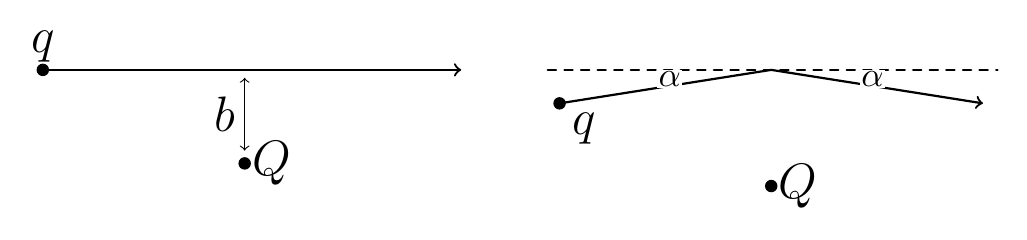
\begin{tikzpicture}[scale=1.25,transform shape,line cap=round,line join=round,every node/.style={inner sep=1pt}]
  \begin{scope}
    \coordinate (qL) at (0,0);
    \coordinate (QL) at (2.05,-0.95);
    \fill (qL) circle (1.8pt);
    \node[font=\Large,above=1pt] at (qL) {$q$};
    \draw[->,thick] (qL) -- (4.25,0);
    \fill (QL) circle (1.8pt);
    \node[font=\Large,right=1pt] at (QL) {$Q$};
    \draw[<->] (2.05,-0.08) -- (2.05,-0.82);
    \node[font=\Large,left=2pt,fill=white,inner sep=0.5pt] at (2.05,-0.45) {$b$};
  \end{scope}
  \begin{scope}[xshift=5.25cm]
    \coordinate (qR) at (0,-0.34);
    \coordinate (V) at (2.15,0);
    \coordinate (Rend) at (4.30,-0.34);
    \coordinate (QR) at (2.15,-1.18);
    \draw[dashed,thick] (-0.12,0) -- (4.45,0);
    \draw[thick] (qR) -- (V);
    \draw[->,thick] (V) -- (Rend);
    \fill (qR) circle (1.8pt);
    \node[font=\Large] at (0.25,-0.60) {$q$};
    \fill (QR) circle (1.8pt);
    \node[font=\Large,right=1pt] at (QR) {$Q$};
    \node[font=\normalsize,fill=white,inner sep=0.4pt] at (1.12,-0.095) {$\alpha$};
    \node[font=\normalsize,fill=white,inner sep=0.4pt] at (3.18,-0.095) {$\alpha$};
  \end{scope}
\end{tikzpicture}
\end{center}
\begin{solution}
记
\[
  C=\frac{qQ}{4\pi\varepsilon_0m} .
\]
粒子受固定电荷的库仑加速度大小为
\[
  a=\frac{|C|}{r^2} .
\]
非相对论 Larmor 公式给出
\[
  P=\frac{q^2a^2}{6\pi\varepsilon_0c^3}
  =\frac{q^2C^2}{6\pi\varepsilon_0c^3}\frac1{r^4} .
\]
\begin{enumerate}
  \item 直线路径取
  \[
    \mathbf r(t)=vt\hat{\mathbf x}+b\hat{\mathbf y},
    \qquad r^2=v^2t^2+b^2 .
  \]
  因此
  \[
  \begin{aligned}
    E_1&=\int_{-\infty}^{\infty}P\,\mathrm dt \\
    &=\frac{q^2C^2}{6\pi\varepsilon_0c^3}
      \int_{-\infty}^{\infty}\frac{\mathrm dt}{(v^2t^2+b^2)^2} .
  \end{aligned}
  \]
  利用
  \[
    \int_{-\infty}^{\infty}\frac{\mathrm dt}{(v^2t^2+b^2)^2}
    =\frac{\pi}{2vb^3},
  \]
  得
  \[
    \boxed{E_1=\frac{q^4Q^2}{192\pi^2\varepsilon_0^3m^2c^3vb^3}} .
  \]

  \item 以折点为原点沿每段轨迹量弧长 $s\geq0$。两段贡献相同，且到固定电荷的距离满足
  \[
    r^2(s)=s^2+b^2-2bs\sin\alpha .
  \]
  因此
  \[
    E_2=\frac{q^2C^2}{6\pi\varepsilon_0c^3}\frac{2}{v}
    \int_0^\infty\frac{\mathrm ds}{(s^2+b^2-2bs\sin\alpha)^2} .
  \]
  保留到 $\alpha$ 的一阶，
  \[
    \frac1{(s^2+b^2-2bs\sin\alpha)^2}
    =\frac1{(s^2+b^2)^2}
    +\frac{4bs\alpha}{(s^2+b^2)^3}+O(\alpha^2) .
  \]
  又
  \[
    \int_0^\infty\frac{\mathrm ds}{(s^2+b^2)^2}=\frac{\pi}{4b^3},
    \qquad
    \int_0^\infty\frac{s\,\mathrm ds}{(s^2+b^2)^3}=\frac{1}{4b^4} .
  \]
  所以
  \[
    \frac{2}{v}\int_0^\infty\frac{\mathrm ds}{(s^2+b^2-2bs\sin\alpha)^2}
    =\frac{\pi}{2vb^3}+\frac{2\alpha}{vb^3}+O(\alpha^2) .
  \]
  与 $E_1$ 比较得
  \[
    \boxed{E_2=E_1\left(1+\frac{4\alpha}{\pi}+O(\alpha^2)\right)} ,
  \]
  因而
  \[
    \boxed{\frac{E_2-E_1}{E_1}=\frac{4\alpha}{\pi}+O(\alpha^2)} .
  \]
\end{enumerate}
\end{solution}
\end{question}
